\chapter{Basic Statistics}

You live near a freeway, and someone asks you, ``How fast do cars on that freeway drive?''

You say ``Pretty fast.''

And they say, ``Can you be more specific?''

And you point your radar speed reader at a car, and say ``That one is going 32.131 meters per second.''

And they say, ``I don't want to know about that specific car. I want to know about all the cars.''

So, you spend the day beside the freeway measuring the speed of every
car that goes by.  And you get a list of a thousand numbers. Here is part of the
list:

\begin{tabular}{c | c | c}
30.462 m/s  & 29.550 m/s & 29.227 m/s \\
37.661 m/s  & 27.899 m/s & 28.113 m/s \\
24.382 m/s & 35.668 m/s & 43.797 m/s \\
31.312 m/s & 37.637 m/s & 30.891 m/s
\end {tabular}

There are 12 numbers here.  We say that there are 12 \textit{samples}.\index{samples}

\section{Mean}

We often talk about the \textit{average} of a set of samples when we
are talking about the \textit{mean}.  To get the mean, you sum up the
samples and divide that number by the number of samples.\index{mean}

The numbers in that table sum to $388.599$.  If you divide that by 12,
you find that the mean of those samples is 32.217 m/s.

We typically use the greek letter $\mu$ (``mu'') to represent the mean. So if you have a set of samples $x_1, x_2, \ldots, x_n$:

$$ \mu = \frac{1}{n} \sum_{i=1}^n x_i$$

This may be the first time you are seeing a summation ($\sum$).  The equation above is equivalent to:\index{summation symbol}

$$ \mu = \frac{1}{n} \left(x_1 + x_2 + \ldots + x_n\right)$$

\begin{Exercise}[title={Mean Grade}, label=grades_mean]

  Teachers often use the mean for grading.  For example, if you took
  six quizzes in a class, your final grade might be the mean of the six
  scores.  Find the mean of these six grades: 87, 91, 98, 65, 87, 100.

\end{Exercise}
\begin{Answer}[ref=grades_mean]

  $$\mu =\frac{1}{6} \left(87 + 91 + 98 + 65 + 87 + 100 \right) = 88$$

\end{Answer}

If you tell your friend ``I measured the speed of 1000 cars, and the
mean is 31.71 m/s'', your friend will wonder ``Are most of the speeds
clustered around 31.71? Or are they all over the place and just happen
to have a mean of 31.71?'' To answer this question we use variance.

\section{Variance}

If you have $n$ samples $x_1, x_2, \ldots, x_n$ that have a mean of $\mu$, the \textit{variance} is defined to be:\index{variance}

$$v = \frac{1}{n}\sum_{i = 1}^{n} \left(x_i - \mu\right)^2$$

That is, you figure out how far each sample is from the median, you
square that, and then you take the mean of all those squared
distances.

\begin{tabular} {c | c | c}

  $x$ & $x - \mu$ & $(x - \mu)^2$\\
  \hline
30.462 & -1.755 & 3.079 \\
29.550 & -2.667 & 7.111\\
29.227 & -2.990 & 8.938\\
37.661 & 5.444 & 29.642\\
27.899 & -4.318 & 18.642\\
28.113 & -4.104 & 16.839 \\
24.382 & -7.835 & 61.381 \\
35.668 & 3.451 & 11.912 \\
43.797 & 11.580 & 134.106\\
31.312 & -0.905 & 0.818\\
37.637 & 5.420 & 29.381\\
30.891 & -1.326 & 1.757\\
\hline
$\sum x = 386.599$ & & $\sum (x - \mu)^2 = 323.605$\\
mean = 32.217 & & variance = 26.967
\end{tabular}

Thus, the variance of the 12 samples is 26.967.  Bigger variances mean
that the samples are spread widely; small variances indicate that the
samples are clustered neatly around the mean.

Notice that most of the data points deviate from the my by 1 to 5
m/s. Isn't it odd that the variance is a big number like 26.967?
Remember that it represents the average of the squares. Sometimes, to
get a better feel for how far the samples are from the mean, we use
the square root of the variance, which is called \textit{the standard
  deviation}.

The standard deviation of your 12 samples would be $\sqrt{26.9677} =
  5.193$ m/s.

The standard deviation is used to figure out if something is an
outlier. For example, if you are asked``That car that just sped
past. Was it going freakishly fast?'' You might respond, ``No, it was
within a standard deviation of the mean.'' or ``Yes, it's speed was 2
standard deviations more than the mean. They will probably get a ticket.''

Just a $\mu$ usually represents the mean. $\sigma$ usually represents
the standard deviation.  So $\sigma^2$ represents the variance.

\begin{Exercise}[title={Variance of Grades}, label=grades_variance]

  Now find the variance for your six grades.  As a reminder, they were: 87, 91, 98, 65, 87, 100.

  What is your standard deviation?

\end{Exercise}
\begin{Answer}[ref=grades_variance]

  The mean of your grades is $88$.

  The variance, then is

  $$\sigma^2 = \frac{1}{6} \left((87 - 88)^2 + (91 - 88)^2 + (98 - 88)^2 + (61 - 88)^2 + (87 - 88)^2 + (100 - 88)^2 \right) = \frac{981 \frac{1}{3}}{6} \approx 81.78$$

  The standard deviation is the square root of that: $\sigma = 9.043$ points.
  
\end{Answer}


\section{Median}

Sometimes you want to know where the middle is. For example, you want
to know the speed at which half the cars are going faster and half are
going slower. To get the median, you sort your samples from smallest
to largest. If you have an odd number of samples, the one in the
middle is the median.  If you have an even number of samples, we take
the mean of the two numbers in the middle.\index{median}

In our example, you would sort your numbers and find the two in the middle:

\begin{tabular}{c}
24.382\\
27.899\\
28.113\\
29.227\\
29.550\\
\hline
\textbf{30.462}\\
\textbf{30.891}\\
\hline 
31.312\\
35.668\\
37.637\\
37.661\\
43.797\\
\end{tabular}

You take the mean of the two middle numbers: $(30.462 + 30.891)/2 =
30.692$.  The median speed would be 30.692 m/s.

Medians are often used when a small number of samples really skew the
mean. For example, income statistics usually use the median income
because a few hundred billionares raise the mean a lot.

\begin{Exercise}[title={Median Grade}, label=grades_median]

  Find the median of your six grades: 87, 91, 98, 65, 87, 100.

\end{Exercise}
\begin{Answer}[ref=grades_median]

  In order the grades are 65, 87, 87, 91, 98, 100.  The middle two are 87
  and 91. The mean of those is 89. (Speed trick: The mean of two numbers is the
  number that is half-way between.)
  
 \end{Answer}


\section{Histograms}

A histogram is a bar chart that shows how many samples are in each
group. In our example, we group cars by speed. Maybe we count the
number of cars going between 30 and 32 m/s.  And then we count the
cars going between 32 and 34 m/2.  And then we make a bar chart from
that data.\index{histograms}

Your 1000 cars would break up into these groups:

\begin{tabular}{ c | c }
0 - 2 m/s & 0 cars \\
2 - 4 m/s & 0 cars \\
4 - 6 m/s & 0 cars \\
\ldots & \ldots \\
20 - 22 m/s & 0 cars \\
22 - 24 m/s & 0 cars \\
24 - 26 m/s & 65 cars \\
26 - 28 m/s & 160 cars \\
28 - 30 m/s & 175 cars \\
30 - 32 m/s & 168 cars \\
32 - 34 m/s & 150 cars \\
34 - 36 m/s & 114 cars \\
36 - 38 m/s & 79 cars \\
38 - 40 m/s & 52 cars \\
40 - 42 m/s & 20 cars \\
42 - 44 m/s & 12 cars \\
44 - 46 m/s & 4 cars \\
46 - 48 m/s & 1 cars \\
48 - 50 m/s & 0 cars \\
\end{tabular}

Now you make a bar chart from that:

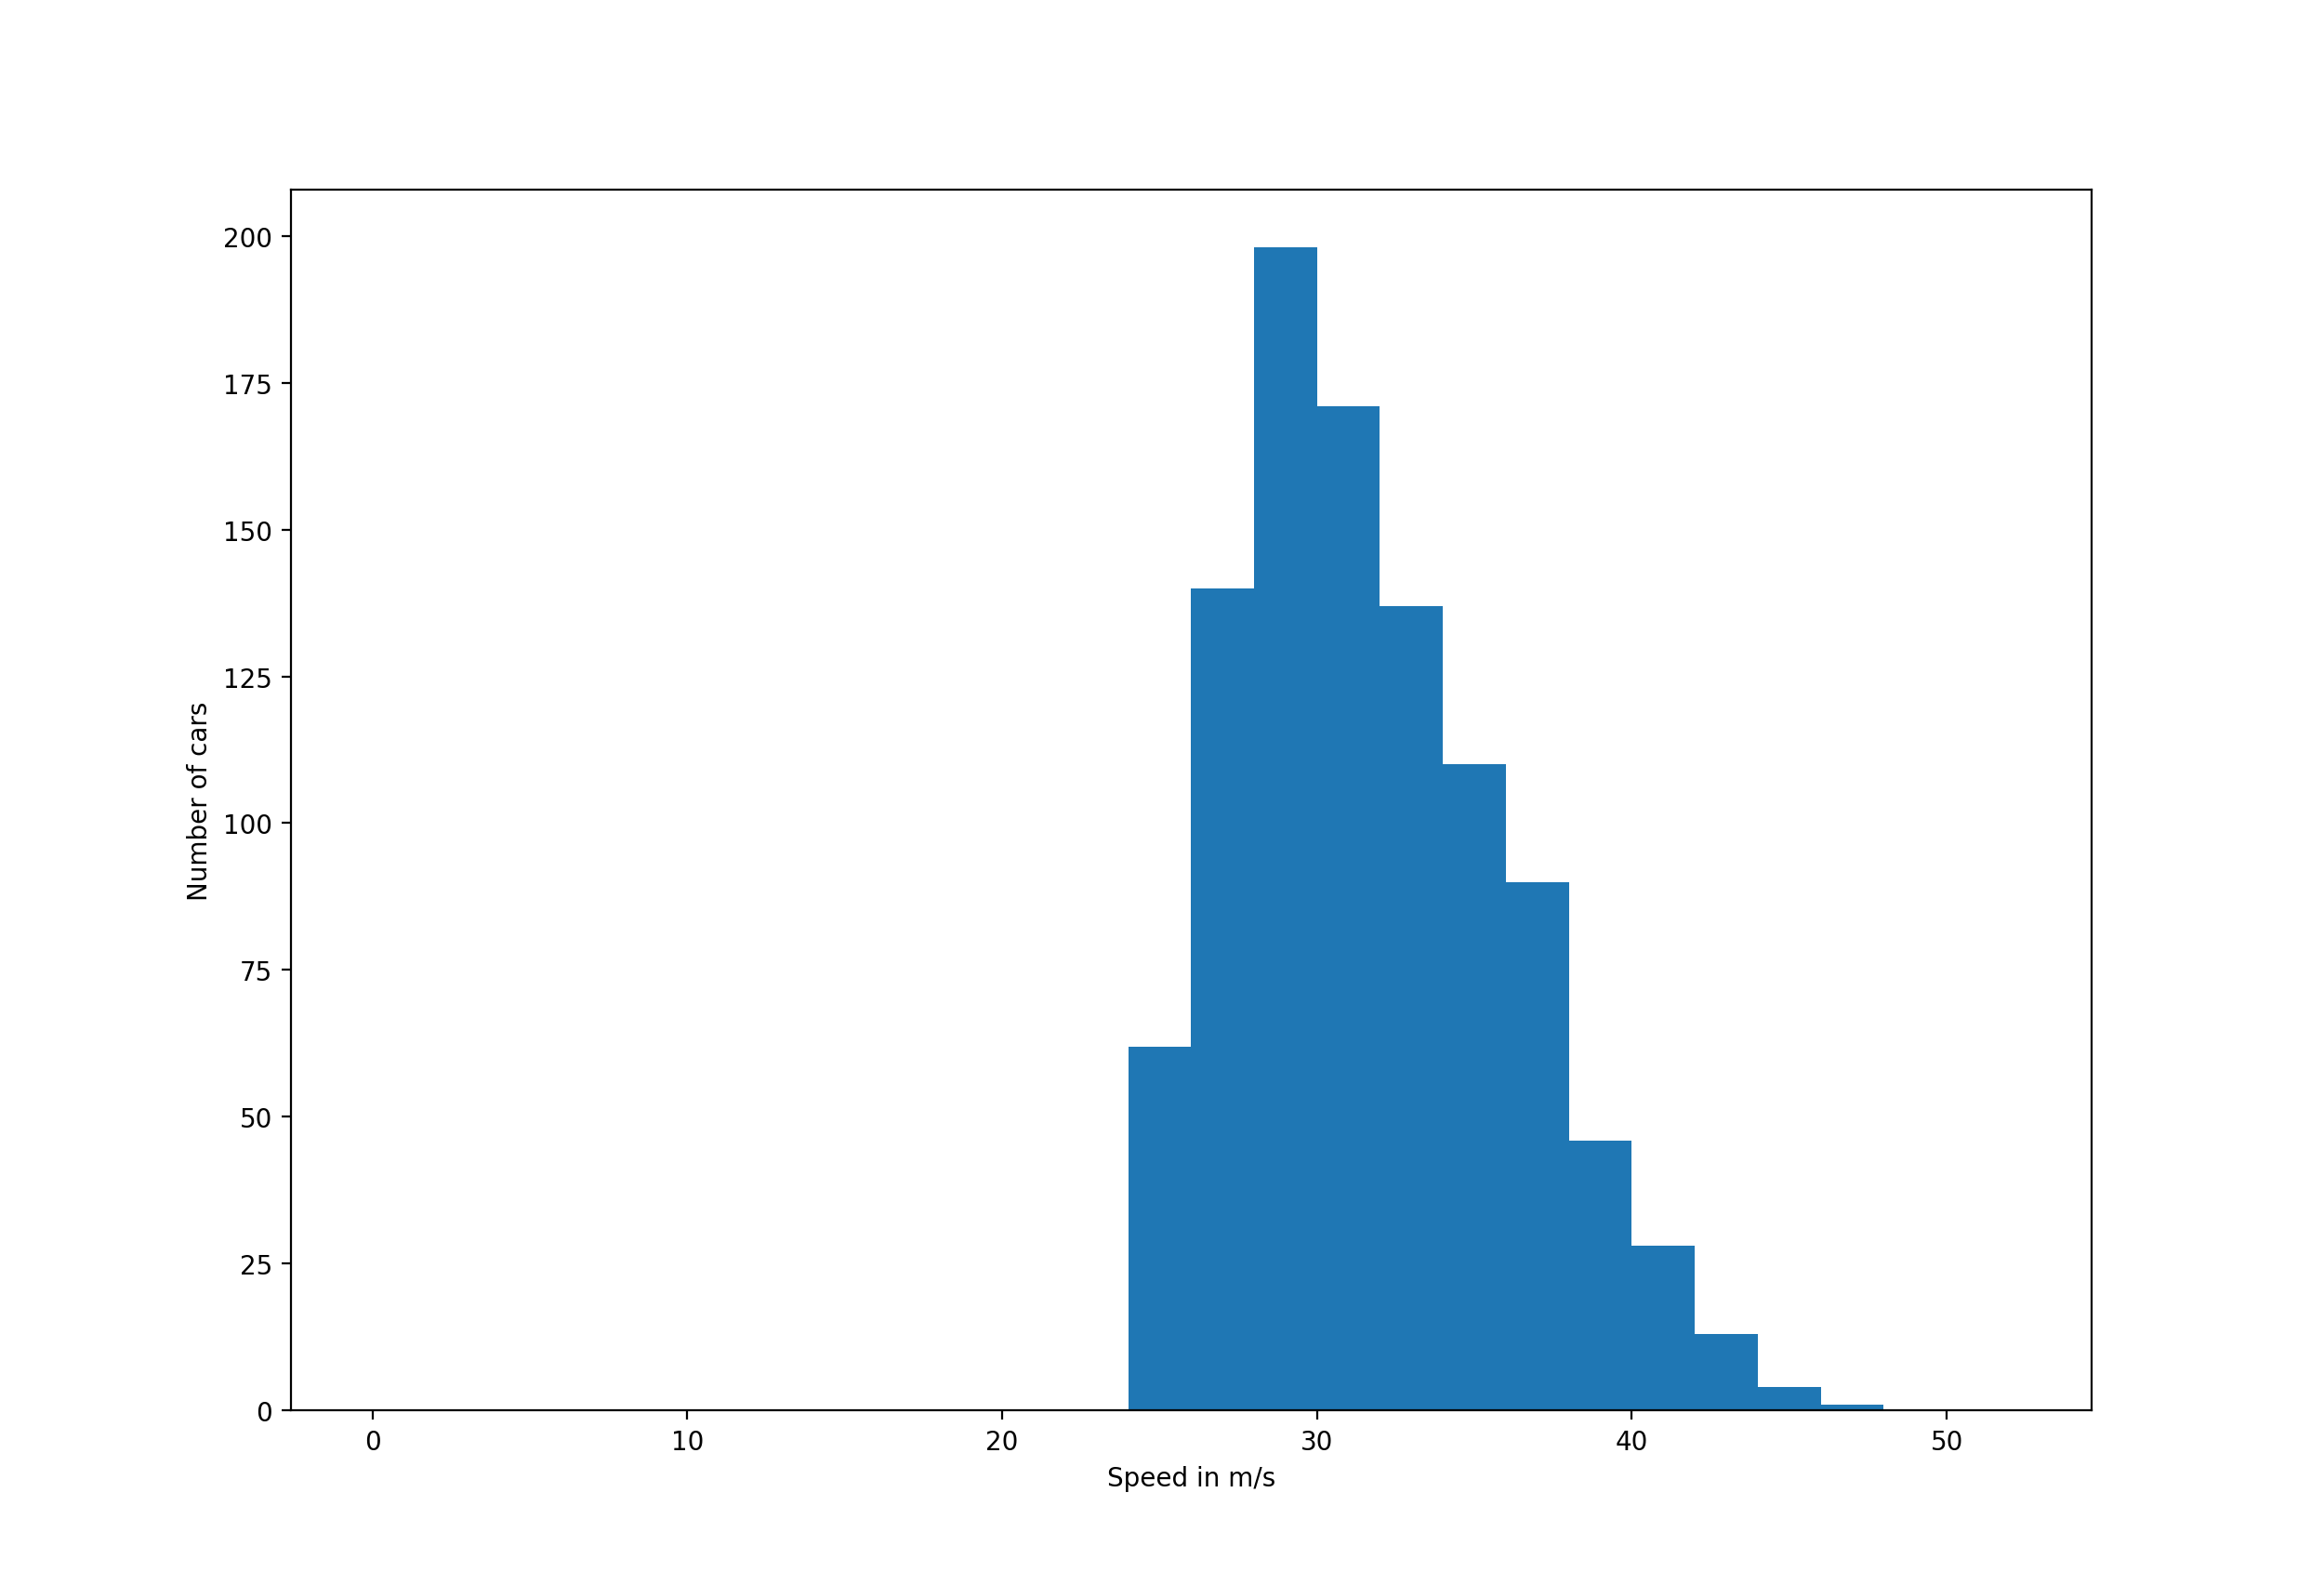
\includegraphics[width=\textwidth] {speed_histo.png}

Often a histogram will tell the story of the data. Here, you can see
that no one is going less than 24 m/s, but a lot of people travel at
30 m/s. There are few people who travel over 40 m/s, but there are a
couple of people who drive a lot faster than anyone else.

\section{Root-Mean-Squared}

Scientists have a mean-like statistic that they love. It is named
quadratic mean, but everyone just calls it Root-Mean-Squared or
RMS. If you have a list of numbers $x_1, x_2, \ldots, x_n$, their RMS
is \index{quadratic mean} \index{root-mean-squared} \index{RMS}

$$\sqrt{\frac{1}{n}\left( x_1^2 + x_2^2 + \ldots + x_n^2 \right)}$$

You are taking the square root of the mean of squares of the samples,
thus the name Root-Mean-Squared.

Using your 12 samples:

\begin{tabular}{c |  c}
  $x$ & $x^2$ \\
  \hline
30.462 & 927.933 \\
29.550 & 873.203\\
29.227 & 854.218\\
37.661 & 1418.351\\
27.899 & 778.354\\
28.113 & 790.341\\
24.382 & 594.482\\
35.668 & 1272.206\\
43.797 & 1918.177\\
31.312 & 980.441\\
37.637 & 1416.544\\
30.891 & 954.254\\
\hline
\multicolumn{1}{r}{Mean of $x^2$} & {1064.875}\\
\multicolumn{1}{r}{RMS} & {32.632}
  \end{tabular}

Why is RMS useful? Let's say that all cars had the same mass $m$, and
you need to know what the average kinetic energy per car is.  If you
know that the RMS of the speeds of the cars is $v_{rms}$, the average kinetic energy for
each car is

$$k = \frac{1}{2}m v_{rms}^2$$

(You don't believe me? Let's prove it. Substitute in the RMS:

$$k = \frac{1}{2}m \sqrt{\frac{1}{n}\left( x_1^2 + x_2^2 + \ldots + x_n^2 \right)}^2$$

The square root and the square cancel each other out:

$$k = \frac{1}{2}m \frac{1}{n}\left( x_1^2 + x_2^2 + \ldots + x_n^2 \right)$$

Use the distributive property:

$$k = \frac{1}{n} \left( \frac{1}{2} m x_1^2 + \frac{1}{2}m x_2^2 + \ldots + \frac{1}{2}m x_n^2 \right)$$


That is all the kinetic energy divided by the number of cars, which is
the mean kinetic enegy per car. Quod erat demonstrandum! (That is a
Latin phrase that means ``which is what I was trying
demonstrate''. You will sometimes see ``QED'' at the end of a long
mathematic proof.))

Now you are ready for the punchline: kinetic energy and heat are the
same thing. Instead of cars, heat is the kinetic energy of molecules
moving around. More on this soon.
